En esta sección se exponen investigaciones recientes vinculadas al análisis de la percepción pública en entornos digitales, la minería de sentimientos, la detección dinámica de temas y la aplicación de modelos de lenguaje de gran escala (LLMs) en contextos sociopolíticos y electorales. En cada estudio se describen el problema tratado, el objetivo planteado, la metodología empleada, las técnicas aplicadas y los resultados alcanzados.

% ──────────────────────────────────────────────────────────────
%  ANTECEDENTE 1
% ──────────────────────────────────────────────────────────────
\cite{pr_alvarez2023llm_political} publicaron el artículo titulado \citetitle{pr_alvarez2023llm_political} en la revista \textit{Frontiers in Political Science}, el cual traducido al español significa «Modelos de Lenguaje de Gran Escala y Ciencia Política».
 
Ante la proliferación de herramientas de inteligencia artificial generativa como ChatGPT y la escasa orientación académica sobre su uso responsable en contextos políticos, los autores plantearon la necesidad de ofrecer un marco conceptual claro para integrar los LLMs en la investigación en ciencia política y metodología computacional. El objetivo principal fue examinar las aplicaciones actuales y potenciales de los LLMs en tareas de análisis político, incluyendo clasificación de textos, detección de sentimientos y análisis del discurso electoral.
 
Según la metodología empleada por los autores, se realizó una revisión analítica y sistemática de casos de uso emergentes de LLMs en ciencia política. Se examinaron herramientas como ToxicBERT y la API Perspective para la detección de contenido político sensible. Asimismo, se analizaron flujos de trabajo que combinan Named Entity Recognition (NER) con análisis de sentimientos bajo técnicas de aprendizaje \textit{few-shot}, comparando su desempeño frente a algoritmos separados de NLP.
 
Los resultados mostraron que los LLMs, al integrar el análisis conjunto de entidades y sentimientos en un único modelo, superan en precisión contextual a los algoritmos especializados individuales. Específicamente, se demostró que un LLM con aprendizaje \textit{few-shot} puede identificar simultáneamente a qué actor político se refiere un tweet y el sentimiento expresado hacia él, algo que los sistemas de NER + análisis de sentimientos por separado no logran eficientemente. La Figura \ref{fig:alvarez2023} ilustra el flujo de trabajo propuesto para la generación de contenido político con LLMs en campañas electorales.
 
\begin{figure}[!ht]
    \begin{center}
        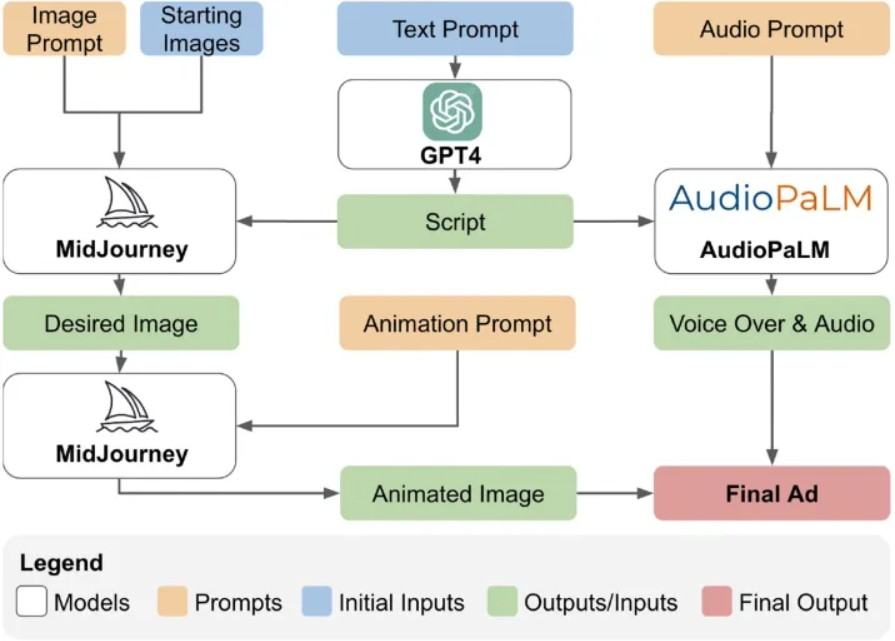
\includegraphics[width=0.85\textwidth]{2/figures/alvarez2023_workflow.jpg}
        \caption[Flujo de trabajo para generación y análisis de contenido político con LLMs]{Flujo de trabajo para la generación y análisis de contenido político mediante LLMs en el contexto de campañas electorales.\\
            Fuente: \cite{pr_alvarez2023llm_political}. \citetitle{pr_alvarez2023llm_political}. (p. 4)}
        \label{fig:alvarez2023}
    \end{center}
\end{figure}
 
Se concluyó que los LLMs representan una herramienta transformadora para la ciencia política computacional, con aplicaciones directas en la clasificación de polaridad política, el monitoreo de narrativas electorales y la detección de discurso de odio en ecosistemas digitales.
 
% ──────────────────────────────────────────────────────────────
%  ANTECEDENTE 2
% ──────────────────────────────────────────────────────────────
\cite{pr_gujral2024llm_elections} publicaron el artículo titulado \citetitle{pr_gujral2024llm_elections}, el cual traducido al español significa «¿Pueden los LLMs Ayudar a Predecir Elecciones? Evidencia (Contraria) de la Democracia más Grande del Mundo».
 
El problema abordado fue la limitación de los métodos convencionales de encuestas de opinión y \textit{exit polls} para capturar en tiempo real la dinámica del sentimiento público en contextos electorales masivos y lingüísticamente diversos. Los autores se preguntaron si los LLMs podían superar a estas metodologías tradicionales al predecir resultados electorales mediante el análisis de grandes volúmenes de publicaciones en redes sociales. El objetivo fue evaluar la capacidad predictiva de LLMs de código abierto aplicados al análisis de sentimientos en tweets relacionados con elecciones legislativas estatales en la India.
 
De acuerdo a la metodología seguida por los autores, se recolectaron publicaciones de la plataforma X (antes Twitter) relacionadas con diferentes elecciones estatales en India. Se aplicaron dos LLMs de código abierto —Llama~2 y Zephyr— mediante técnicas de \textit{prompting} para clasificar el sentimiento de los tweets hacia cada partido político, sin recurrir a \textit{fine-tuning}. Los resultados de sentimiento fueron agregados para generar predicciones de resultados electorales, las cuales fueron comparadas directamente con los resultados reales y con predicciones de encuestas tradicionales. La Figura \ref{fig:gujral2024} muestra la comparación entre las predicciones del modelo LLM y los resultados electorales reales en los estados analizados.
 
\begin{figure}[!ht]
    \begin{center}
        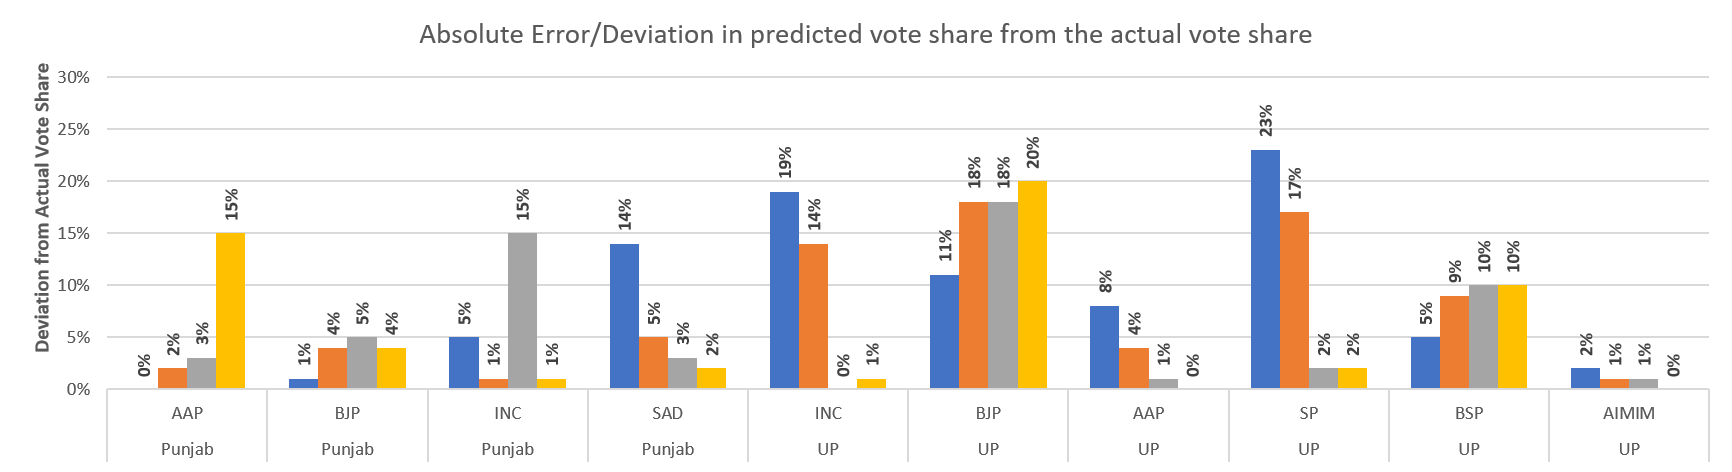
\includegraphics[width=0.82\textwidth]{2/figures/gujral2024_predictions.png}
        \caption[Comparación entre predicciones del modelo LLM y resultados electorales reales en estados de India]{Comparación entre las predicciones basadas en análisis de sentimientos con LLMs y los resultados electorales reales en distintos estados de India.\\
            Fuente: \cite{pr_gujral2024llm_elections}. \citetitle{pr_gujral2024llm_elections}. (p. 6)}
        \label{fig:gujral2024}
    \end{center}
\end{figure}
 
Los resultados mostraron que los modelos basados en LLMs lograron predicciones más cercanas a los resultados electorales reales que los \textit{exit polls} y encuestas de opinión tradicionales en varios de los estados analizados. Sin embargo, también se identificaron limitaciones importantes, como la baja penetración de internet en ciertas regiones y la diversidad lingüística del electorado, factores que restringen la representatividad de los datos de redes sociales.
 
Se concluyó que el análisis de sentimientos con LLMs constituye una perspectiva novedosa y prometedora para la inteligencia electoral, aunque su aplicabilidad varía según el contexto sociocultural y el nivel de digitalización de la población.
 
% ──────────────────────────────────────────────────────────────
%  ANTECEDENTE 3
% ──────────────────────────────────────────────────────────────
\cite{pr_mendonca2025bertopic_political} publicaron el artículo titulado \citetitle{pr_mendonca2025bertopic_political}, el cual traducido al español significa «Modelado del Discurso Político con Sentence-BERT y BERTopic».
 
El problema central identificado por los autores fue la ausencia de metodologías capaces de rastrear dinámicamente la evolución de los temas en el discurso político digital, y de medir la influencia de los valores morales en su longevidad. Ante la limitación de modelos estáticos de detección de temas como LDA, los autores se propusieron diseñar un marco de evolución temática que integre modelos de embeddings semánticos con teorías del comportamiento político. El objetivo fue analizar la duración y las dimensiones morales de los temas presentes en la actividad de Twitter del 117.º Congreso de los Estados Unidos.
 
Según la metodología empleada por los autores, se recolectaron tweets publicados por miembros del Congreso durante el período legislativo estudiado. Se aplicaron embeddings semánticos mediante el modelo Sentence-BERT (variante \textit{all-MiniLM-L6-v2}) para representar el contenido de cada tweet en un espacio vectorial de alta dimensión. Posteriormente, se realizó reducción de dimensionalidad con UMAP y clustering con HDBSCAN dentro del framework BERTopic, permitiendo la detección automática de temas sin necesidad de definir previamente su número. Para rastrear la evolución temporal, se implementó el módulo de \textit{dynamic topic modeling} de BERTopic, que segmenta los datos en ventanas de tiempo y re-entrena las representaciones de cada período. Finalmente, se integró la Teoría de Fundamentos Morales (MFT) para medir qué valores morales dominan en los temas más duraderos. La arquitectura del marco de trabajo propuesto se ilustra en la Figura \ref{fig:mendonca2025}.
 
\begin{figure}[!ht]
    \begin{center}
        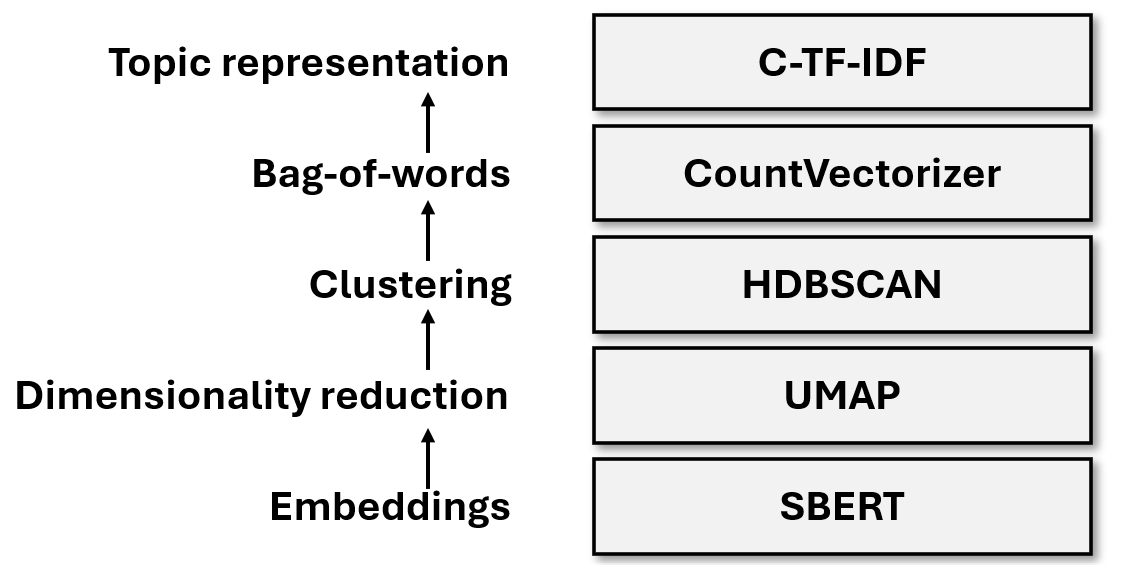
\includegraphics[width=0.88\textwidth]{2/figures/mendonca2025_framework.png}
        \caption[Marco de trabajo para detección dinámica de temas y análisis de fundamentos morales en Twitter político]{Marco de trabajo para la detección dinámica de temas con BERTopic y el análisis de fundamentos morales aplicado al discurso político en Twitter.\\
            Fuente: \cite{pr_mendonca2025bertopic_political}. \citetitle{pr_mendonca2025bertopic_political}. (p. 5)}
        \label{fig:mendonca2025}
    \end{center}
\end{figure}
 
Los resultados revelaron que, si bien los temas generales tienden a permanecer estables a lo largo del tiempo, los temas más granulares se disuelven rápidamente, limitando su influencia en el discurso político sostenido. Además, se encontró que los fundamentos morales de «Cuidado» y «Lealtad» predominan en los temas de mayor longevidad, mientras que las diferencias partidarias se manifiestan en distintas estrategias de encuadre moral.
 
Se concluyó que la integración de BERTopic con marcos teóricos como la MFT permite una comprensión más profunda de las dinámicas del discurso político en ecosistemas digitales, siendo una metodología directamente aplicable a sistemas de inteligencia electoral que requieran monitoreo de narrativas en tiempo real.
 
% ──────────────────────────────────────────────────────────────
%  ANTECEDENTE 4
% ──────────────────────────────────────────────────────────────
\cite{pr_janssens2025bertopic_llm} publicaron el artículo titulado \citetitle{pr_janssens2025bertopic_llm}, el cual traducido al español significa «Reducción de Temas Asistida por LLMs para BERTopic en Datos de Redes Sociales».
 
El problema abordado fue que el framework BERTopic, aunque efectivo para la extracción de temas a partir de grandes corpus, genera un número excesivo de temas semánticamente superpuestos cuando se aplica a datos de redes sociales, caracterizados por ser cortos, ruidosos y dispersos. Esta proliferación de temas redundantes dificulta la interpretación de los resultados y limita la utilidad práctica del modelo en contextos de monitoreo político. El objetivo fue desarrollar un método de reducción de temas automático, interpretable, reproducible y escalable que combine las fortalezas de BERTopic con la capacidad semántica de los LLMs.
 
Según la metodología empleada por los autores, el proceso se diseñó en dos etapas principales. En la primera, BERTopic genera un conjunto inicial de temas mediante embeddings de transformers y clustering con HDBSCAN. Cada tema es representado por sus diez palabras clave principales (extraídas mediante c-TF-IDF) o por una etiqueta generada por un LLM. En la segunda etapa, estas representaciones son entregadas como entrada a un LLM, que recibe instrucciones para identificar y fusionar iterativamente los temas semánticamente similares hasta alcanzar un número objetivo de temas. Se evaluaron cuatro LLMs distintos: GPT-4o-mini, Llama3-8b, Gemma3-12b y Qwen3-30b-a3b, aplicados sobre tres datasets de redes sociales: tweets de Trump, tweets de COVID-19 y tweets de ciberbullying. La Figura \ref{fig:janssens2025} ilustra el pipeline propuesto por los autores, comparando el proceso de reducción asistida por LLM frente al método estándar de BERTopic.
 
\begin{figure}[!ht]
    \begin{center}
        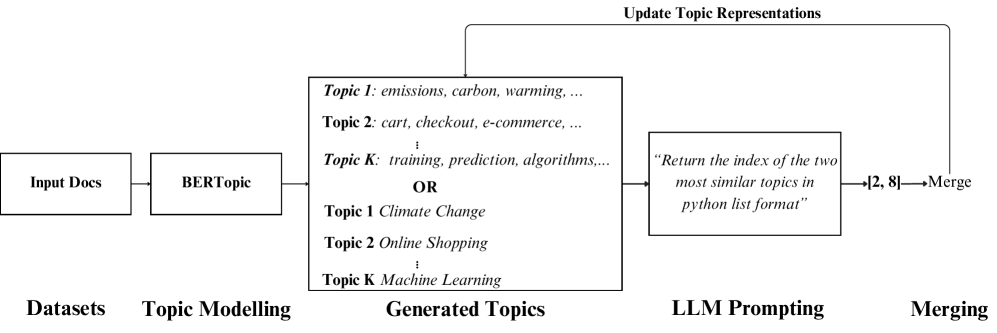
\includegraphics[width=0.90\textwidth]{2/figures/janssens2025_pipeline.png}
        \caption[Pipeline de reducción de temas asistida por LLMs combinada con BERTopic para datos de redes sociales]{Pipeline propuesto que combina BERTopic para la generación inicial de temas y LLMs para la reducción iterativa de temas superpuestos en datos de redes sociales.\\
            Fuente: \cite{pr_janssens2025bertopic_llm}. \citetitle{pr_janssens2025bertopic_llm}. (p. 4)}
        \label{fig:janssens2025}
    \end{center}
\end{figure}
 
Los resultados evidenciaron mejoras significativas en coherencia y diversidad temática respecto al método interno de reducción de BERTopic (parámetro \texttt{nr\_topics}), siendo GPT-4o-mini el modelo que obtuvo los resultados más consistentes en los tres datasets evaluados. El método propuesto demostró ser reproducible y metodológicamente transparente, resolviendo una importante brecha en la literatura de modelado de temas para datos de redes sociales.
 
Se concluyó que la integración de LLMs como asistentes de reducción temática en el pipeline de BERTopic constituye una solución viable y escalable para el análisis de grandes volúmenes de datos políticos digitales, con aplicaciones directas en sistemas de detección dinámica de temas electorales.
 
% ──────────────────────────────────────────────────────────────
%  ANTECEDENTE 5
% ──────────────────────────────────────────────────────────────
\cite{pr_chen2024combating_misinformation} publicaron el artículo titulado \citetitle{pr_chen2024combating_misinformation} en la revista \textit{AI Magazine}, el cual traducido al español significa «Combatiendo la Desinformación en la Era de los LLMs: Oportunidades y Desafíos».
 
El problema central abordado por los autores fue el crecimiento exponencial de la desinformación en plataformas digitales, especialmente en contextos electorales, y la insuficiencia de los métodos tradicionales de detección —basados en características lingüísticas y redes de propagación— para hacer frente a la velocidad y sofisticación del contenido falso generado en la actualidad. El objetivo fue mapear sistemáticamente el rol dual de los LLMs en el ecosistema de la desinformación: como amenaza potencial al ser capaces de generar noticias falsas convincentes, y como herramienta de defensa al poder detectarlas y verificarlas de manera automatizada.
 
Según la metodología empleada por los autores, se realizó una revisión sistemática de la literatura reciente sobre detección y generación de desinformación mediante LLMs. Se construyeron y analizaron datasets de noticias falsas generadas por modelos como GPT-3.5, evaluando la dificultad de su detección tanto por humanos como por sistemas automáticos. Asimismo, se examinaron arquitecturas de verificación basadas en \textit{retrieval-augmented generation} (RAG) y técnicas de \textit{fact-checking} automatizado. La Figura \ref{fig:chen2024} muestra el marco conceptual de oportunidades y desafíos identificado por los autores en torno al uso de LLMs para combatir la desinformación.
 
\begin{figure}[!ht]
    \begin{center}
        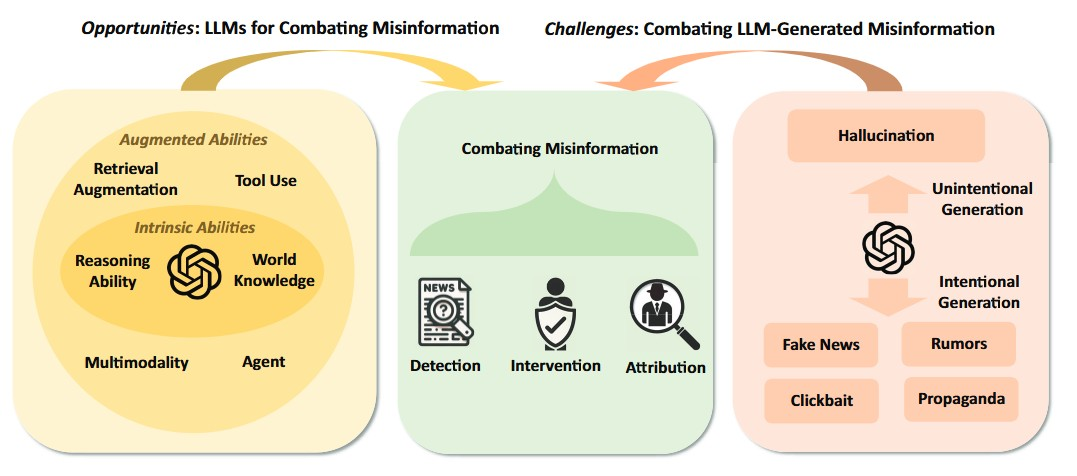
\includegraphics[width=0.80\textwidth]{2/figures/chen2024_framework.jpg}
        \caption[Marco conceptual de oportunidades y desafíos de los LLMs en la detección de desinformación electoral]{Marco conceptual que ilustra el rol dual de los LLMs como generadores y detectores de desinformación en procesos electorales.\\
            Fuente: \cite{pr_chen2024combating_misinformation}. \citetitle{pr_chen2024combating_misinformation}. (p. 3)}
        \label{fig:chen2024}
    \end{center}
\end{figure}
 
Los resultados del estudio mostraron que los LLMs de última generación, como GPT-4, alcanzan alta precisión en la detección de noticias falsas incluso cuando el contenido falso fue generado después de su fecha de corte de conocimiento, lo que sugiere que los modelos aprenden patrones estilísticos y argumentativos del contenido desinformativo más allá de su conocimiento factual. Sin embargo, también se identificaron vulnerabilidades importantes: el contenido falso generado por LLMs resulta significativamente más difícil de detectar que el generado por humanos, tanto para sistemas automáticos como para lectores humanos.
 
Se concluyó que la integración de módulos de verificación basados en LLMs es fundamental en cualquier sistema de inteligencia electoral que analice la percepción pública en ecosistemas digitales, dado que la desinformación condiciona directamente la opinión ciudadana y los resultados de las encuestas en línea.
 
% ──────────────────────────────────────────────────────────────
%  ANTECEDENTE 6
% ──────────────────────────────────────────────────────────────
\cite{pr_alvi2023twitter_election_review} publicaron el artículo titulado \citetitle{pr_alvi2023twitter_election_review} en la revista \textit{PeerJ Computer Science}, cuya traducción en nuestro idioma es «En las Fronteras de los Datos de Twitter y el Análisis de Sentimientos en la Predicción Electoral: Una Revisión».
 
El problema identificado fue la ausencia de una síntesis comprehensiva y actualizada que integre los avances en NLP, aprendizaje automático y datos de redes sociales para la predicción de resultados electorales. A pesar del crecimiento sostenido de publicaciones en este campo, existía una brecha en la sistematización de metodologías, fuentes de datos y métricas de evaluación utilizadas. El objetivo de los autores fue evaluar el estado del arte de forma sistemática, identificando tendencias, enfoques dominantes, limitaciones recurrentes y vacíos en la literatura sobre predicción electoral mediante análisis de sentimientos en Twitter.
 
Según la metodología empleada por los autores, se realizó una revisión sistemática de la literatura, seleccionando y analizando estudios relevantes sobre predicción electoral con datos de Twitter. Se examinaron trabajos que utilizaron enfoques que van desde clasificadores léxicos y SVM hasta redes neuronales profundas y modelos basados en transformers como BERT y RoBERTa. Para cada estudio se documentó el conjunto de datos utilizado, el método de análisis de sentimientos, el modelo de predicción y las métricas de evaluación reportadas. La Figura \ref{fig:alvi2023} muestra la evolución cronológica de los enfoques metodológicos identificados en la revisión, desde métodos léxicos hasta LLMs.
 
\begin{figure}[!ht]
    \begin{center}
        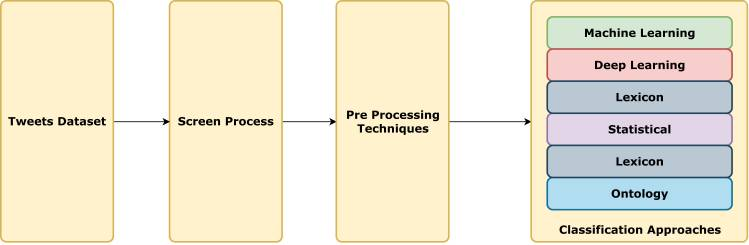
\includegraphics[width=0.85\textwidth]{2/figures/alvi2023_evolution.jpg}
        \caption[Evolución cronológica de los enfoques de análisis de sentimientos para predicción electoral en Twitter]{Evolución de los enfoques metodológicos en la predicción electoral mediante análisis de sentimientos en Twitter, desde métodos léxicos hasta modelos de lenguaje de gran escala.\\
            Fuente: \cite{pr_alvi2023twitter_election_review}. \citetitle{pr_alvi2023twitter_election_review}. (p. 8)}
        \label{fig:alvi2023}
    \end{center}
\end{figure}
 
Los resultados de la revisión evidenciaron una evolución sostenida hacia modelos de mayor precisión: los clasificadores basados en SVM lograron exactitudes entre el 66\% y el 86\%, mientras que los modelos de aprendizaje profundo y los basados en transformers alcanzaron rangos de exactitud del 86\% al 97\% según el contexto electoral analizado. Se identificó además que la incorporación de características de sentimiento, más allá del mero volumen de menciones, mejora consistentemente el poder predictivo de los modelos.
 
Se concluyó que la combinación de análisis de sentimientos con técnicas de NLP avanzado constituye una línea de investigación madura y en plena expansión, con aplicaciones directas en sistemas de inteligencia electoral. Este trabajo valida la pertinencia del enfoque metodológico adoptado en la presente investigación.
 
% ──────────────────────────────────────────────────────────────
%  ANTECEDENTE 7
% ──────────────────────────────────────────────────────────────
\cite{pr_islam2025latent_topic} publicaron el artículo titulado \citetitle{pr_islam2025latent_topic}, el cual traducido al español significa «Síntesis Latente de Temas: Aprovechando los LLMs para el Análisis de Publicidad Electoral».
 
El problema abordado fue la incapacidad de los modelos de tópicos tradicionales —como LDA y el propio BERTopic sin supervisión semántica— para capturar estructuras discursivas latentes y jerarquías temáticas complejas en grandes corpus dinámicos de publicidad política en redes sociales. Los autores se preguntaron si era posible construir automáticamente, sin intervención humana ni conjunto semilla inicial, una taxonomía coherente e interpretable de temas políticos a partir de datos no etiquetados de campañas electorales. El objetivo fue desarrollar un framework de síntesis temática iterativa basado en LLMs para analizar las estrategias de publicidad política en redes sociales durante las elecciones presidenciales de los Estados Unidos de 2024.
 
Según la metodología empleada por los autores, se construyó y publicó un dataset curado de anuncios de campaña de las elecciones presidenciales de 2024. El proceso metodológico se estructuró en múltiples etapas: primero, se realizaron embeddings de los anuncios y se aplicó clustering de densidad siguiendo el enfoque de BERTopic. Luego, en lugar de generar etiquetas con c-TF-IDF, se utilizó un LLM para producir etiquetas semánticamente ricas para cada cluster. A continuación, el framework construye iterativamente una taxonomía de temas, partiendo de cero y fusionando o refinando etiquetas en cada iteración hasta alcanzar una estructura jerárquica coherente, sin requerir un conjunto de temas predefinido. La arquitectura completa del framework propuesto se ilustra en la Figura \ref{fig:islam2025}.
 
\begin{figure}[!ht]
    \begin{center}
        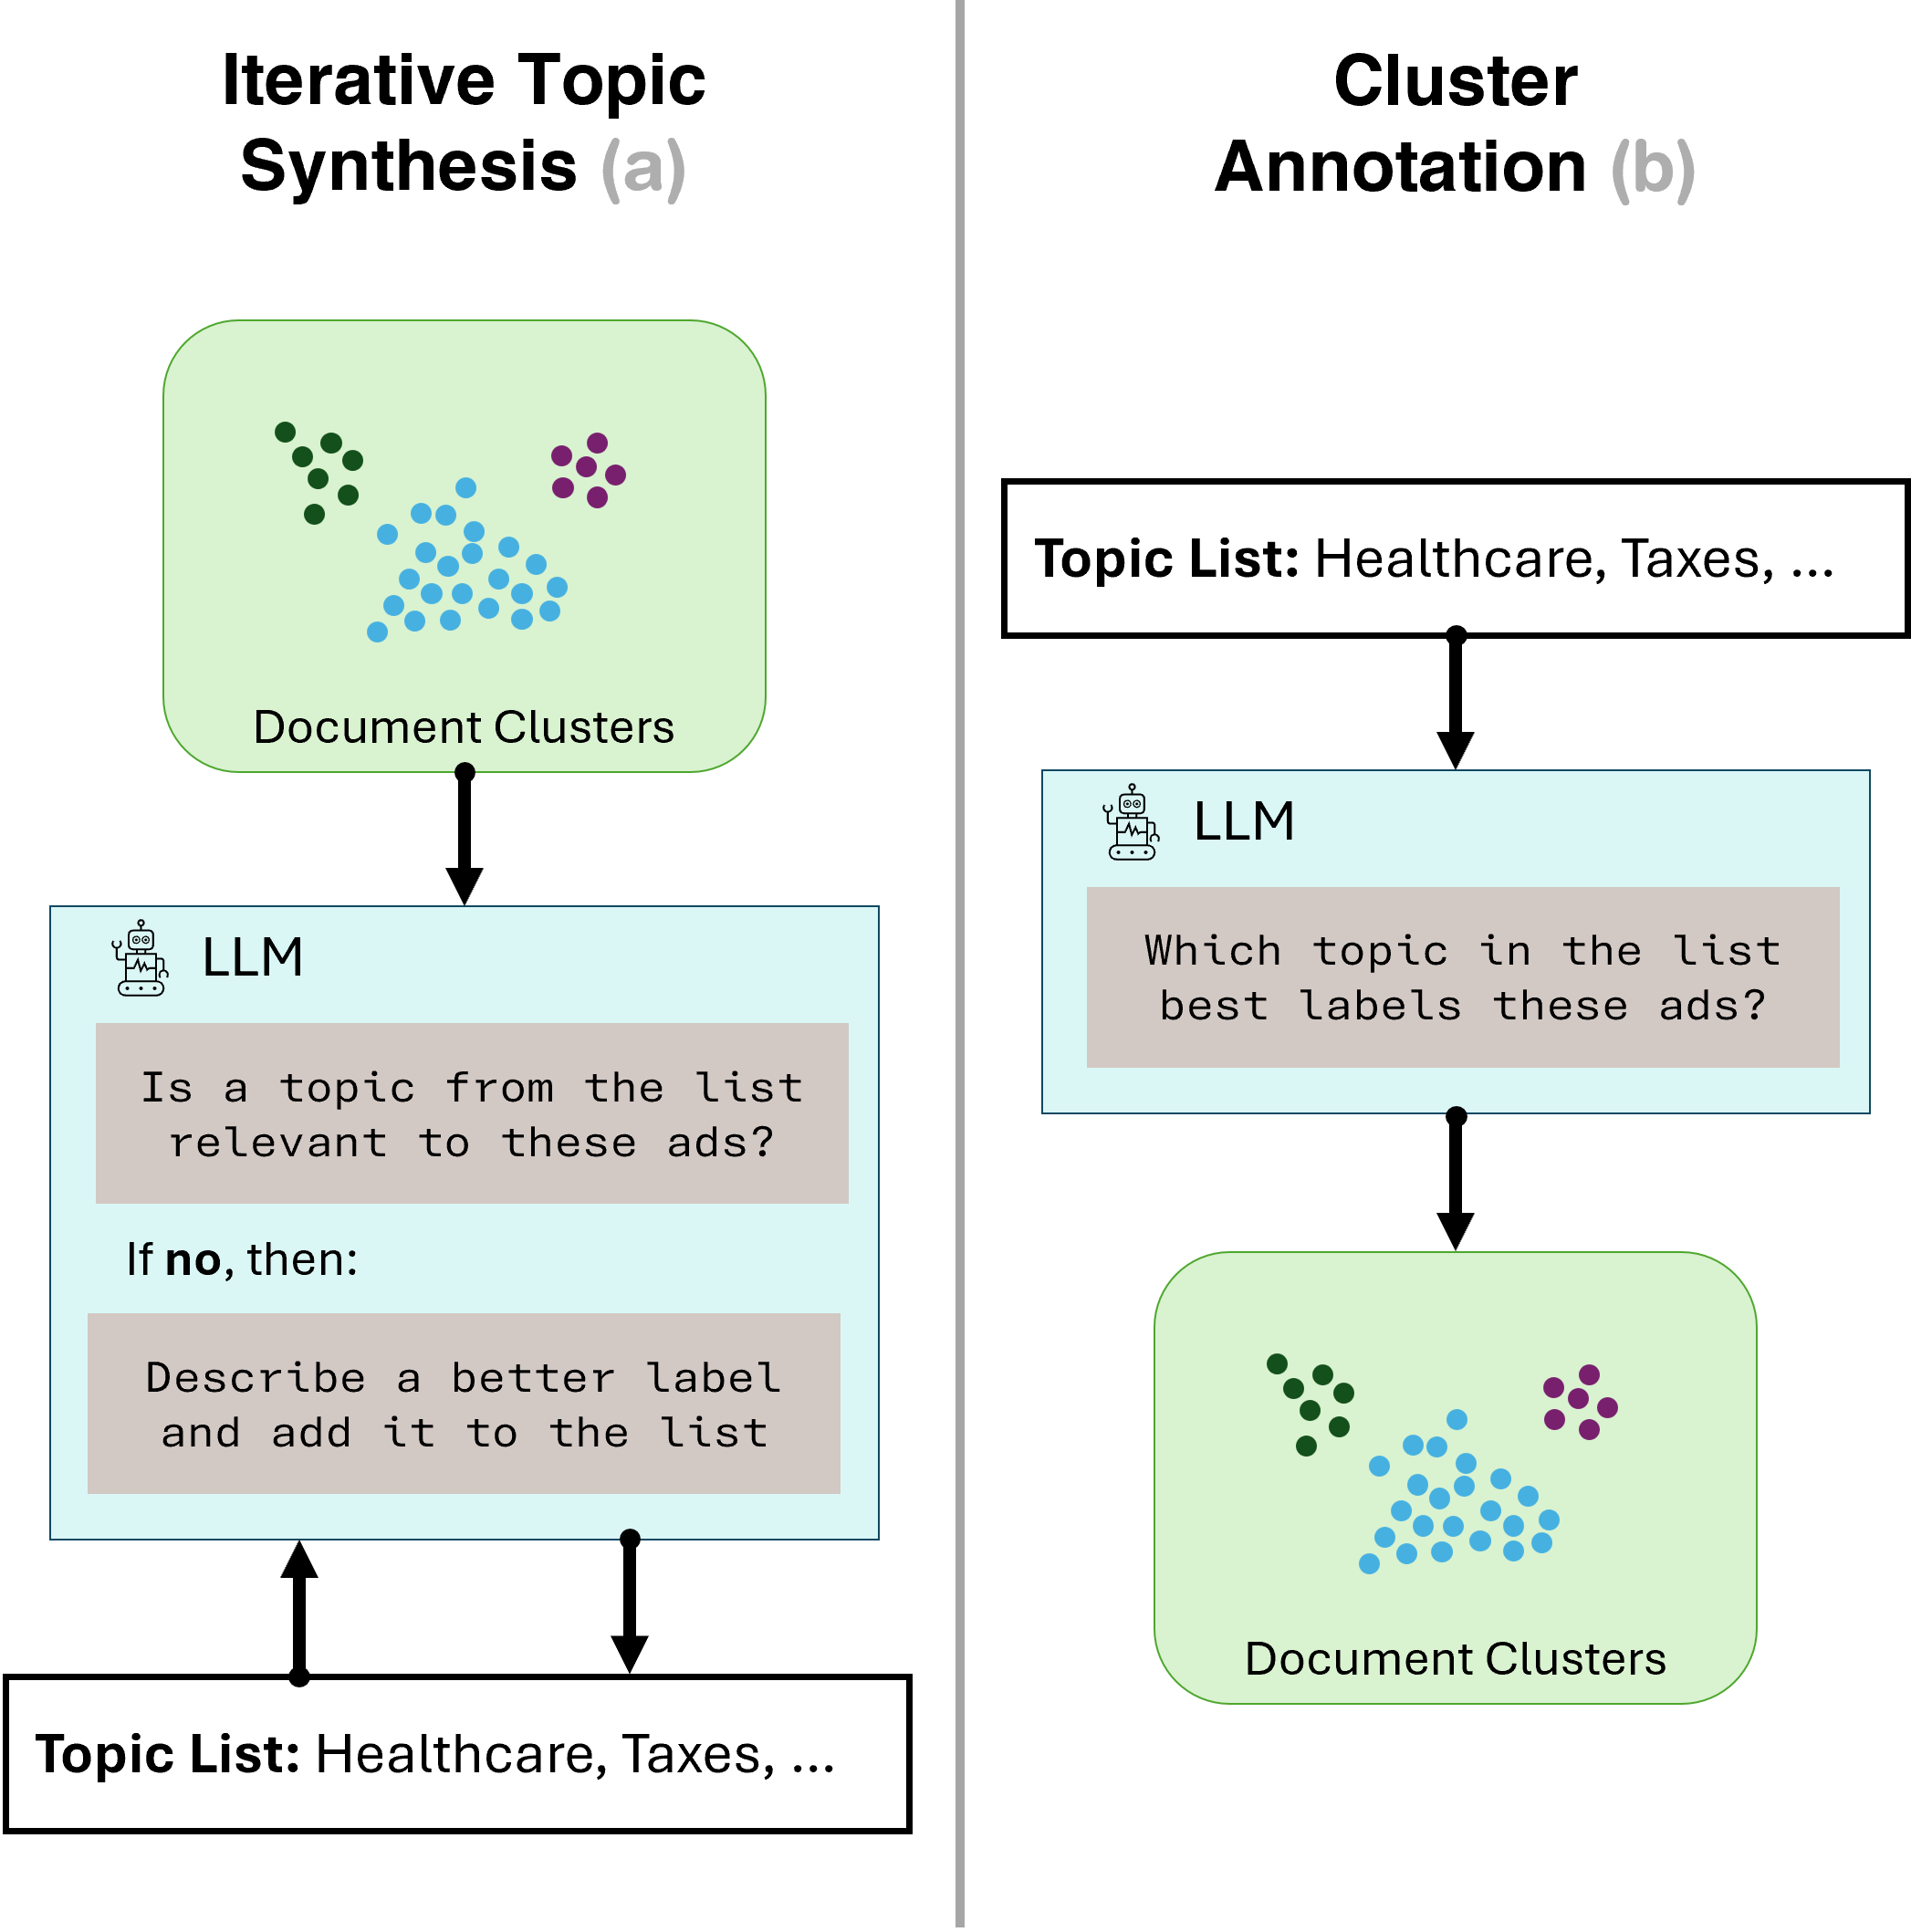
\includegraphics[width=0.92\textwidth]{2/figures/islam2025_architecture.png}
        \caption[Arquitectura del framework de síntesis temática iterativa con LLMs para análisis de publicidad política]{Arquitectura del framework de síntesis de temas latentes mediante LLMs, aplicado al análisis de publicidad política en las elecciones presidenciales de EE.UU. 2024.\\
            Fuente: \cite{pr_islam2025latent_topic}. \citetitle{pr_islam2025latent_topic}. (p. 4)}
        \label{fig:islam2025}
    \end{center}
\end{figure}
 
Los resultados de la evaluación demostraron que el mecanismo de síntesis iterativa produce etiquetas de temas más consistentes y mejor alineadas con el juicio humano que los modelos clásicos de tópicos y que el etiquetado directo mediante LLMs en un único paso (\textit{single-shot}). Anotadores expertos en ciencias sociales computacionales validaron cualitativamente la coherencia y granularidad de la taxonomía generada, confirmando su utilidad para el análisis de estrategias de microfocalización electoral.
 
Se concluyó que este framework de síntesis temática iterativa es altamente aplicable a sistemas de monitoreo electoral en tiempo real, donde la identificación rápida y automática de temas emergentes —sin necesidad de etiquetado manual previo— representa una ventaja fundamental. Este trabajo es directamente relevante para la presente investigación, ya que valida la viabilidad de construir sistemas de inteligencia electoral capaces de detectar dinámicamente los temas relevantes que moldean la percepción actual proyectada por los medios de comunicación en ecosistemas digitales.